\begin{frame}{Phänomenologie}
\textbf{Supraleitung}: Ab einer Sprungtemperatur $T_{\mathup{C}}$ fällt elektrischer Widerstand auf $\SI{0}{\ohm}$ \\
\begin{columns}
\begin{column}{0.49\textwidth}
  \begin{figure}
    \fbox{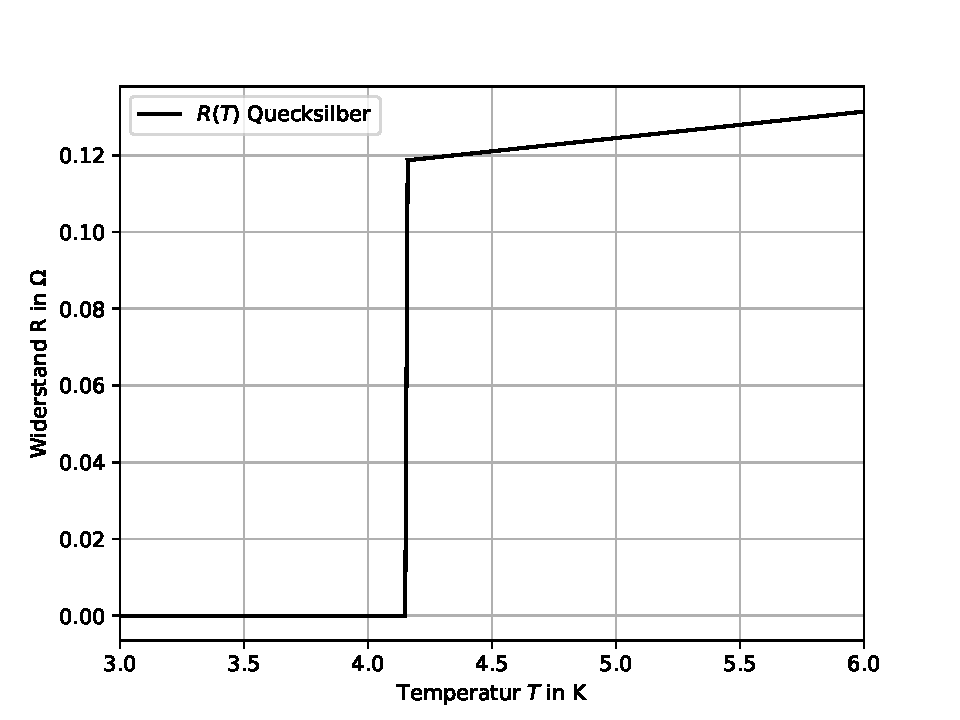
\includegraphics[width = \textwidth]{quecksilber_supra.pdf}}
    \label{fig: hg_supraleitung}
  \end{figure}
\end{column}
\begin{column}{0.49\textwidth}
\begin{itemize}
  \item Quecksilber: $T_{\mathup{C}} = \SI{4.15}{\kelvin}$
  \item Aluminium: $T_{\mathup{C}} = \SI{1.17}{\kelvin}$
  \item \ce{TlCaBaCuO}
\end{itemize}
\end{column}
\end{columns}




\end{frame}



\begin{frame}{Meißner-Ochsenfeld-Effekt}
\begin{columns}
\begin{column}{0.49\textwidth}
  \begin{figure}
    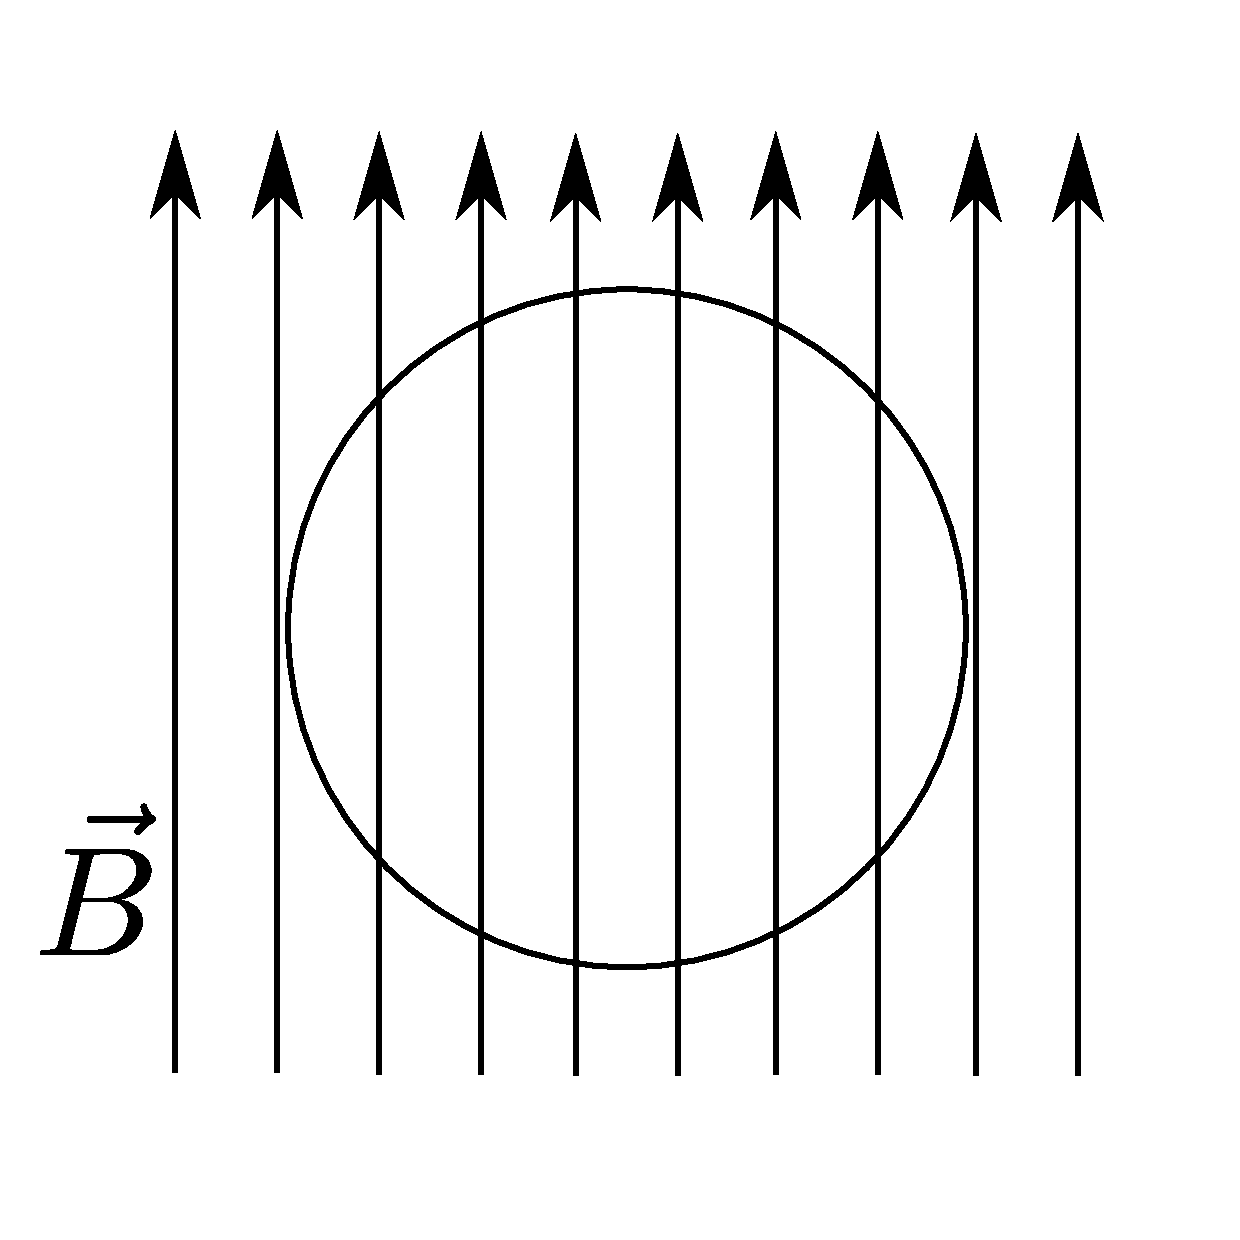
\includegraphics[width = \textwidth]{supra_1.pdf}
    \caption{Normale Leitung $T > T_{C}$}
    \label{fig: bfeld_normale_leitung}
  \end{figure}
\end{column}
\begin{column}{0.49\textwidth}
  \begin{figure}
    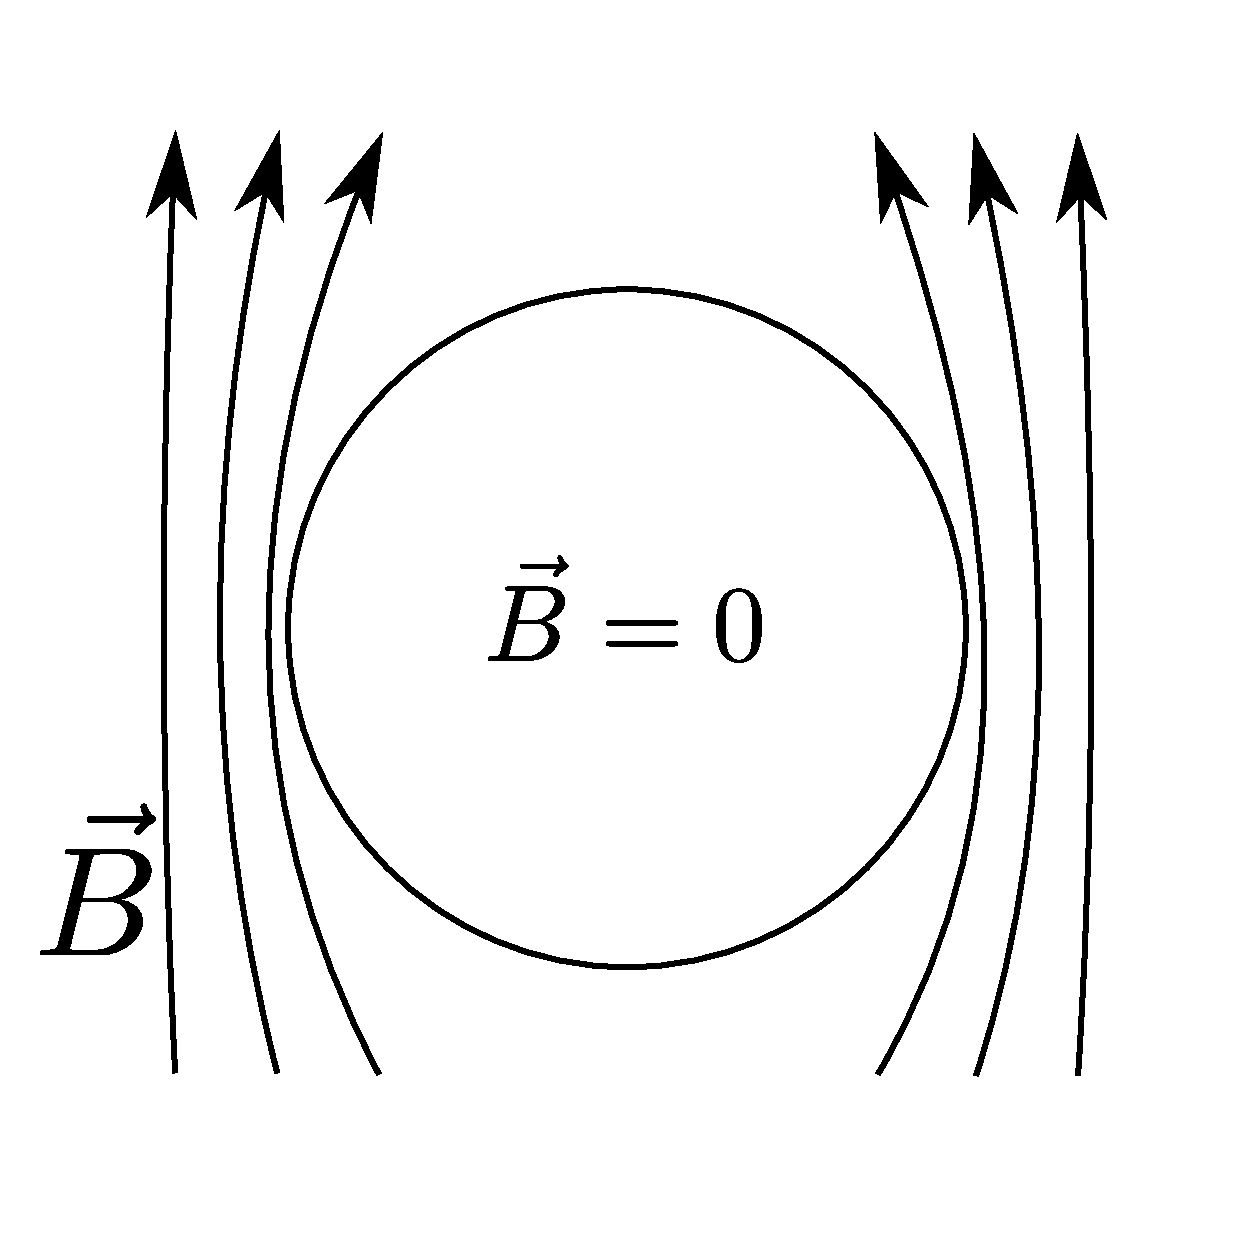
\includegraphics[width = \textwidth]{supra_2.pdf}
    \caption{Supraleitung $T < T_{C}$}
    \label{fig: bfeld_supraleitung}
  \end{figure}
\end{column}
\end{columns}
\end{frame}
